\documentclass{cquptformat}
\usepackage{wallpaper}
\ULCornerWallPaper{0.7085}{figures/insignia.png}% 校徽水印,注释掉可去除
\pagestyle{empty}% 在整个文档中去除页码

% 文档的标题和信息
\coursename{XXXXXX}		% 课程名称
\coursenum{XXXXXX}		% 课程编号
\place{XXXXXX}			% 实验地点
\exptime{XXXXXX}		% 实验时间
\oninstructor{XXXXXX}	% 校内指导老师
\expname{XXXXXXXXXXXX}	% 实验名称

\begin{document}
	
% 生成封面
\maketitle
\makeatother
\makeatletter

% 实验目的
\section{实验目的}

\begin{enumerate}
	\item 摆脱word排版的折磨
	\item 使用latex完成论文的简要排版
	\item 爽写报告 
\end{enumerate}

% 实验原理
\section{实验原理}

\subsection{使用latex完成实验报告的简单排版}

在使用中只需要掌握latex基本的公式格式(可以使用Axmath、Mathtype等工具转换成latex)、插入单图或双图以及表格的基本使用(使用excel2latex插件)即可。学习时间成本不到1天,便可以罔顾word的格式折磨,尽情挥洒灵感。


\subsubsection{插入图片}
\begin{lstlisting}[language=tex]
	%% 插单图
	\begin{figure}[H]
		\centering
		\includegraphics[width=0.8\textwidth]{figures/11111}
		\caption{22222}
		\label{fig:33333}
	\end{figure}
	
	%% 插双图
	\begin{figure}[ht]
		\centering
		\begin{subfigure}[ht]{0.49\textwidth}
			\centering
			\includegraphics[width=\linewidth]{11111.png}
			\caption{11111}
			\label{fig:11111}
		\end{subfigure}
		\hspace{2pt}%调整图片之间间距
		\begin{subfigure}[ht]{0.49\textwidth}
			\centering
			\includegraphics[width=\linewidth]{22222.png}
			\caption{22222}
			\label{fig:22222}
		\end{subfigure}
		\caption{33333}
		\label{fig:33333}
	\end{figure}
	
\end{lstlisting}

%% 交叉引用——使用\ref{}可对\label{}进行交叉引用。不过要注意编译时需使用xelatex->xelatex,即使用xelatex编译两次才会显示出序号。
如图\ref{fig:lenna}所示,这是使用卷积滤波对图像进行边缘检测的结果对比。

%% 插单图
\begin{figure}[H]
	\centering
	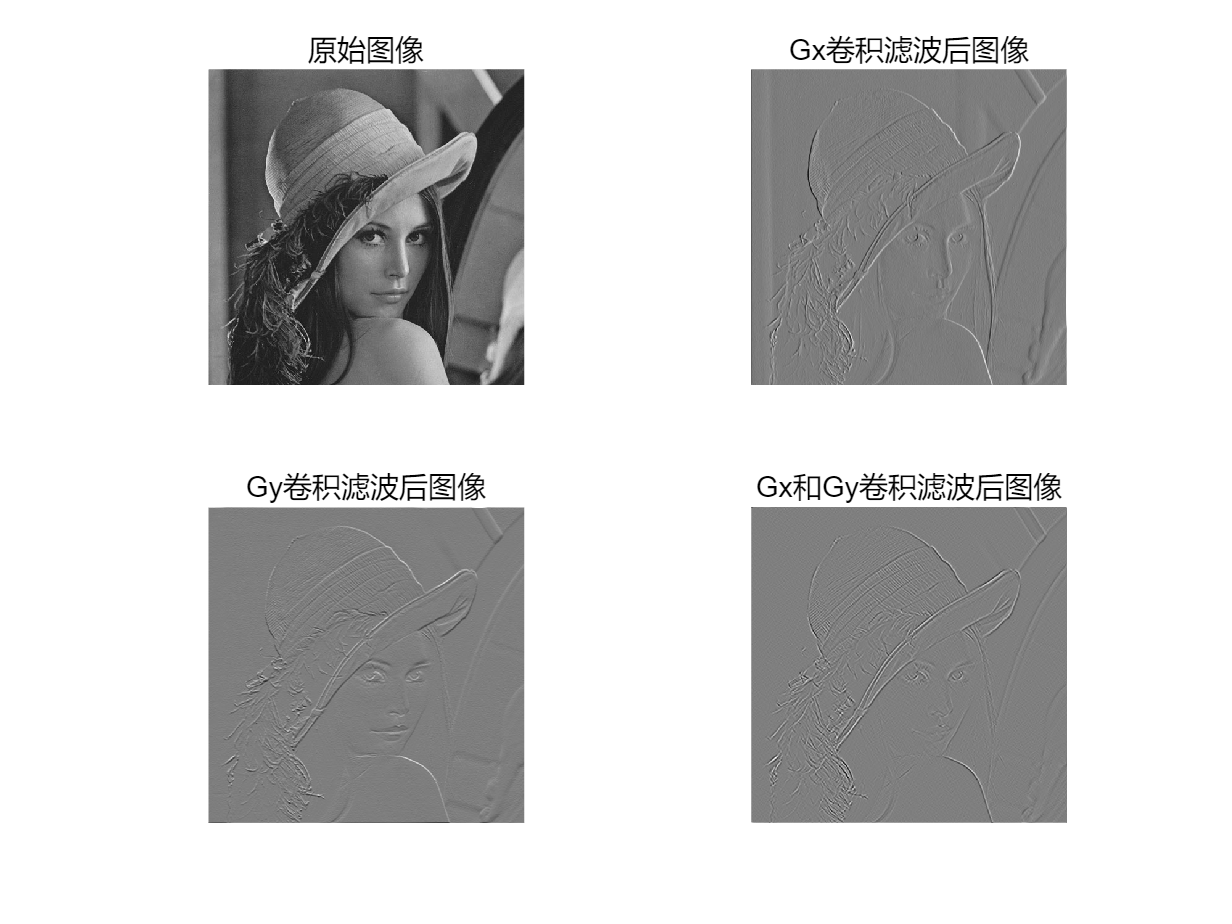
\includegraphics[width=0.8\textwidth]{figures/lenna.png}
	\caption{这是一张照片}
	\label{fig:lenna}
\end{figure}

如图\ref{fig:L1}所示,使用filter格impz法求解出的$h(n)$一致,且函数收敛。如图\ref{fig:R1}所示,$h(n)$零极点均位于单位圆内。
%% 插双图
\begin{figure}[ht]
	\centering
	\begin{subfigure}[ht]{0.49\textwidth}
		\centering
		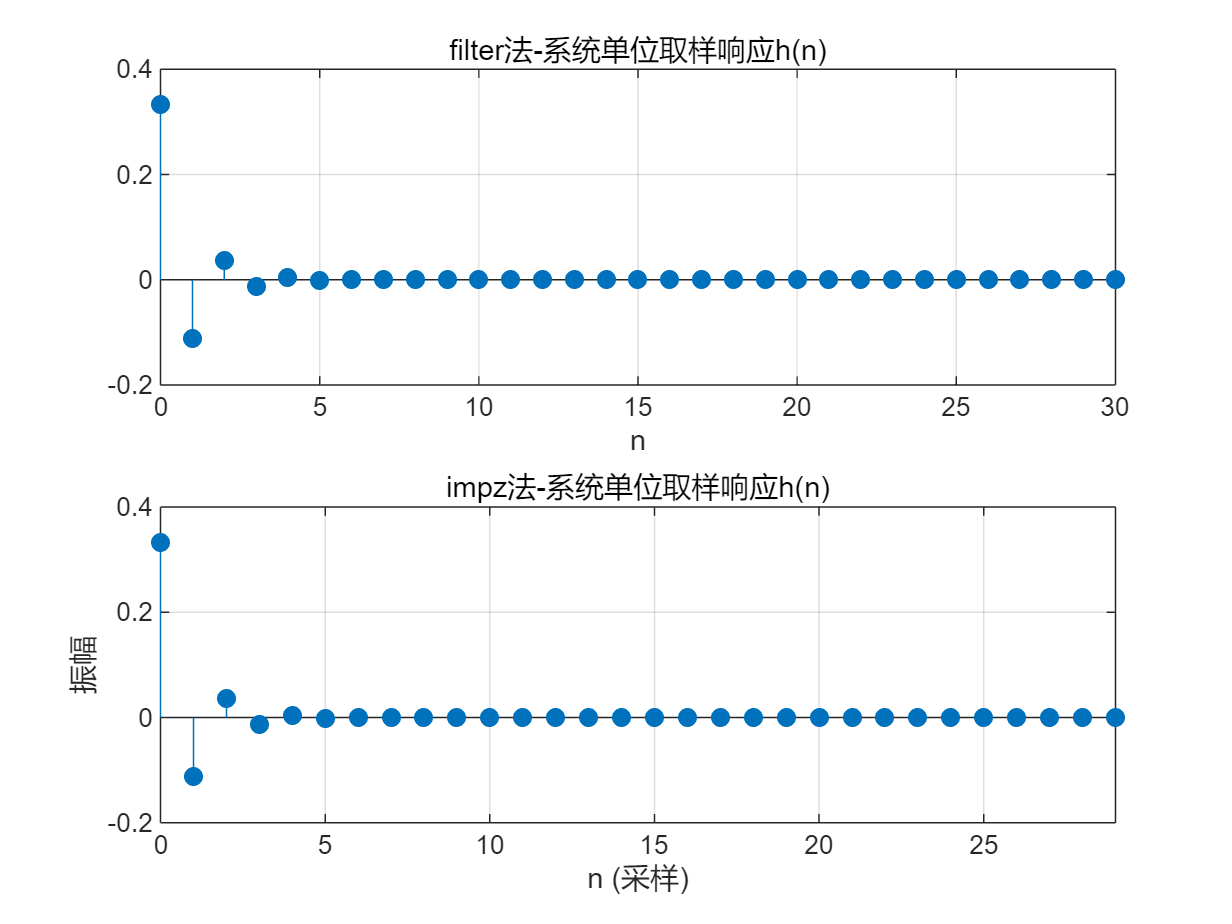
\includegraphics[width=\linewidth]{figures/figure_0.png}
		\caption{左图}
		\label{fig:L1}
	\end{subfigure}
	\hspace{2pt}
	\begin{subfigure}[ht]{0.49\textwidth}
		\centering
		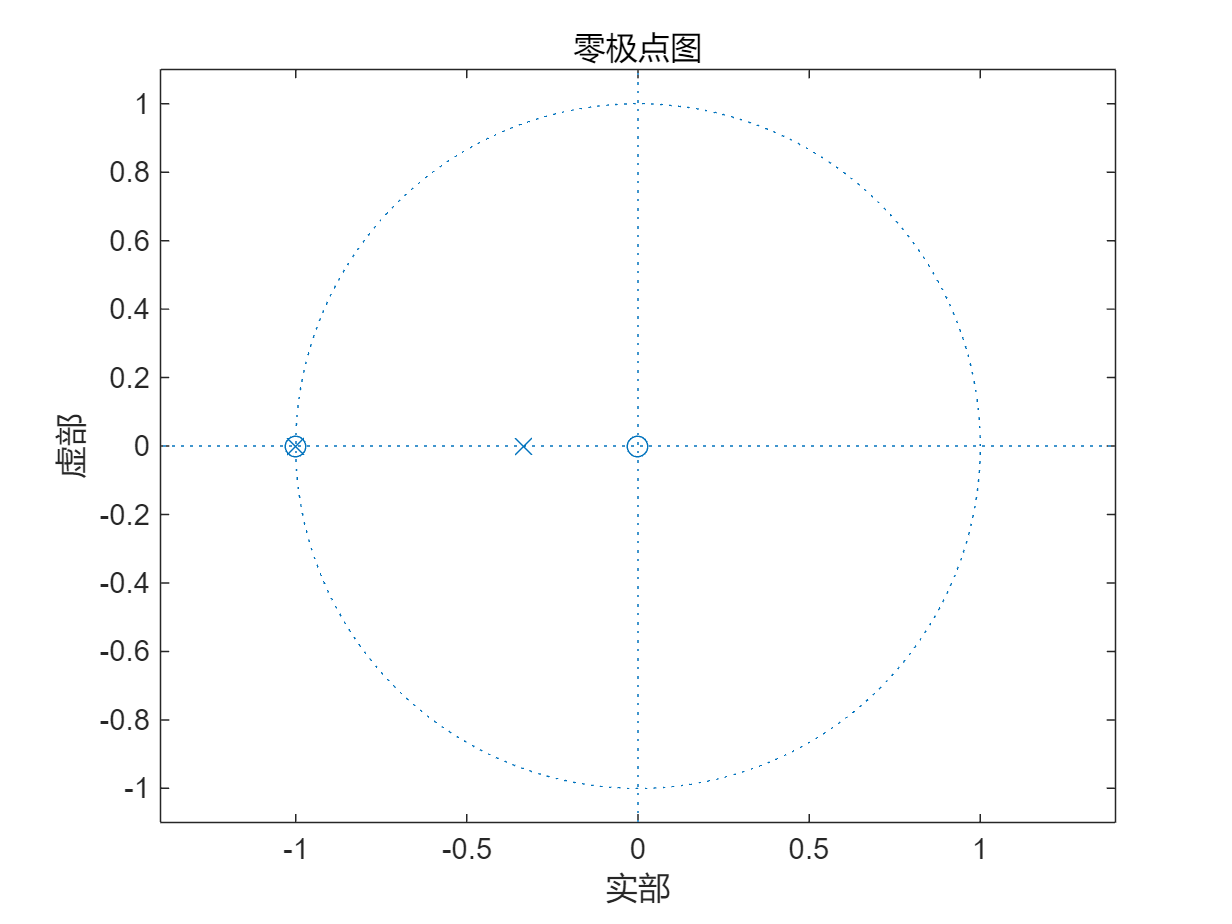
\includegraphics[width=\linewidth]{figures/figure_1.png}
		\caption{右图}
		\label{fig:R1}
	\end{subfigure}
	\caption{双图}
	\label{fig:双图1}
\end{figure}

\newpage

\subsubsection{插入表格}
测试结果如表\ref{tab:测试}所示。


\begin{table}[H]
	\centering
	\caption{测试结果}
	\begin{tabularx}{0.6\linewidth}{>{\centering\arraybackslash}X >{\centering\arraybackslash}X} % 列宽自动调整,内容居中
		\toprule[1.5pt]
		K     & Vo \\
		\midrule
		273uA & 273.00000uV \\
		278uA & 101.70895mV \\
		283uA & 201.62534mV \\
		288uA & 301.54173mV \\
		293uA & 401.45811mV \\
		298uA & 501.37450mV \\
		303uA & 601.29089mV \\
		308uA & 701.20728mV \\
		313uA & 801.123676mV \\
		318uA & 901.04006mV \\
		323uA & 1.00096V \\
		328uA & 1.10087V \\
		333uA & 1.20079V \\
		338uA & 1.30071V \\
		343uA & 1.40062V \\
		348uA & 1.50054V \\
		353uA & 1.60045V \\
		358uA & 1.70037V \\
		363uA & 1.80029V \\
		368uA & 1.9002V \\
		373uA & 2.00012V \\
		\bottomrule[1.5pt]
	\end{tabularx}%
	\label{tab:测试}%
\end{table}

\subsection{使用latex进一步美化布局排版}

熟悉宏包的使用。
进一步完善cls文件的内容,添加更多排版布局优化指令。

% 实验程序及结果分析
\section{实验程序及结果分析}

实验程序将详细说明实验的步骤,结果分析将展示实验数据并进行解释。

如模板所示,本v1.0模板在部分场景仍存在一些不尽如人意的地方。例如:

\quad 1)正文与框线距离过近,且不易于调整。	
						
\quad 2)图像位于页首时,可能会遮挡住上框线。

\quad 3)代码片段跨页时,可能会遮盖住下框线。若且一行内代码过长会超出页面。

等一系列问题。

% 思考题
\section{思考题}
思考题部分将提出一些与实验相关的问题,以供学生思考和讨论。


	
\end{document}